%%%%%%%%%%%%%%%%%%%%%%%%%%%%%%%%%%%%%%%%%
% Article EcoFoG
% Version 2.1 (23/10/2017)
%
% adapté de :
% Stylish Article
% LaTeX Template
% Version 1.0 (31/1/13)
%
% This template has been downloaded from:
% http://www.LaTeXTemplates.com
%
% Original author:
% Mathias Legrand (legrand.mathias@gmail.com)
%
% License:
% CC BY-NC-SA 3.0 (http://creativecommons.org/licenses/by-nc-sa/3.0/)
%
%%%%%%%%%%%%%%%%%%%%%%%%%%%%%%%%%%%%%%%%%


%----------------------------------------------------------------------------------------
%	PACKAGES AND OTHER DOCUMENT CONFIGURATIONS
%----------------------------------------------------------------------------------------

\documentclass[fleqn,10pt]{ArtEcoFoG} % Document font size and equations flushed left

\setcounter{tocdepth}{3} % Show only three levels in the table of contents section: sections, subsections and subsubsections


% Pandoc environments
\usepackage{framed}
\usepackage{fancyvrb}
\providecommand{\tightlist}{%
  \setlength{\itemsep}{0pt}\setlength{\parskip}{0pt}}
\newcommand{\VerbBar}{|}
\newcommand{\VERB}{\Verb[commandchars=\\\{\}]}
\DefineVerbatimEnvironment{Highlighting}{Verbatim}{commandchars=\\\{\}, fontsize=\scriptsize} % Code R
\definecolor{shadecolor}{RGB}{248,248,248}
\newenvironment{Shaded}{\begin{snugshade}}{\end{snugshade}}
\newcommand{\KeywordTok}[1]{\textcolor[rgb]{0.13,0.29,0.53}{\textbf{{#1}}}}
\newcommand{\DataTypeTok}[1]{\textcolor[rgb]{0.13,0.29,0.53}{{#1}}}
\newcommand{\DecValTok}[1]{\textcolor[rgb]{0.00,0.00,0.81}{{#1}}}
\newcommand{\BaseNTok}[1]{\textcolor[rgb]{0.00,0.00,0.81}{{#1}}}
\newcommand{\FloatTok}[1]{\textcolor[rgb]{0.00,0.00,0.81}{{#1}}}
\newcommand{\ConstantTok}[1]{\textcolor[rgb]{0.00,0.00,0.00}{{#1}}}
\newcommand{\CharTok}[1]{\textcolor[rgb]{0.31,0.60,0.02}{{#1}}}
\newcommand{\SpecialCharTok}[1]{\textcolor[rgb]{0.00,0.00,0.00}{{#1}}}
\newcommand{\StringTok}[1]{\textcolor[rgb]{0.31,0.60,0.02}{{#1}}}
\newcommand{\VerbatimStringTok}[1]{\textcolor[rgb]{0.31,0.60,0.02}{{#1}}}
\newcommand{\SpecialStringTok}[1]{\textcolor[rgb]{0.31,0.60,0.02}{{#1}}}
\newcommand{\ImportTok}[1]{{#1}}
\newcommand{\CommentTok}[1]{\textcolor[rgb]{0.56,0.35,0.01}{\textit{{#1}}}}
\newcommand{\DocumentationTok}[1]{\textcolor[rgb]{0.56,0.35,0.01}{\textbf{\textit{{#1}}}}}
\newcommand{\AnnotationTok}[1]{\textcolor[rgb]{0.56,0.35,0.01}{\textbf{\textit{{#1}}}}}
\newcommand{\CommentVarTok}[1]{\textcolor[rgb]{0.56,0.35,0.01}{\textbf{\textit{{#1}}}}}
\newcommand{\OtherTok}[1]{\textcolor[rgb]{0.56,0.35,0.01}{{#1}}}
\newcommand{\FunctionTok}[1]{\textcolor[rgb]{0.00,0.00,0.00}{{#1}}}
\newcommand{\VariableTok}[1]{\textcolor[rgb]{0.00,0.00,0.00}{{#1}}}
\newcommand{\ControlFlowTok}[1]{\textcolor[rgb]{0.13,0.29,0.53}{\textbf{{#1}}}}
\newcommand{\OperatorTok}[1]{\textcolor[rgb]{0.81,0.36,0.00}{\textbf{{#1}}}}
\newcommand{\BuiltInTok}[1]{{#1}}
\newcommand{\ExtensionTok}[1]{{#1}}
\newcommand{\PreprocessorTok}[1]{\textcolor[rgb]{0.56,0.35,0.01}{\textit{{#1}}}}
\newcommand{\AttributeTok}[1]{\textcolor[rgb]{0.77,0.63,0.00}{{#1}}}
\newcommand{\RegionMarkerTok}[1]{{#1}}
\newcommand{\InformationTok}[1]{\textcolor[rgb]{0.56,0.35,0.01}{\textbf{\textit{{#1}}}}}
\newcommand{\WarningTok}[1]{\textcolor[rgb]{0.56,0.35,0.01}{\textbf{\textit{{#1}}}}}
\newcommand{\AlertTok}[1]{\textcolor[rgb]{0.94,0.16,0.16}{{#1}}}
\newcommand{\ErrorTok}[1]{\textcolor[rgb]{0.64,0.00,0.00}{\textbf{{#1}}}}
\newcommand{\NormalTok}[1]{{#1}}
\usepackage{longtable,booktabs}
\usepackage{caption}
% These lines are needed to make table captions work with longtable:
\makeatletter
\def\fnum@table{\tablename~\thetable}
\makeatother
% longtable 2 columns
% https://tex.stackexchange.com/questions/161431/how-to-solve-longtable-is-not-in-1-column-mode-error
\makeatletter
\let\oldlt\longtable
\let\endoldlt\endlongtable
\def\longtable{\@ifnextchar[\longtable@i \longtable@ii}
\def\longtable@i[#1]{\begin{figure}[t]
\onecolumn
\begin{minipage}{0.5\textwidth}\scriptsize
\oldlt[#1]
}
\def\longtable@ii{\begin{figure}[t]
\onecolumn
\begin{minipage}{0.5\textwidth}\scriptsize
\oldlt
}
\def\endlongtable{\endoldlt
\end{minipage}
\twocolumn
\end{figure}}
\makeatother

\usepackage{graphicx,grffile}
\makeatletter
\def\maxwidth{\ifdim\Gin@nat@width>\linewidth\linewidth\else\Gin@nat@width\fi}
\def\maxheight{\ifdim\Gin@nat@height>\textheight0.8\textheight\else\Gin@nat@height\fi}
\makeatother
% Scale images if necessary, so that they will not overflow the page
% margins by default, and it is still possible to overwrite the defaults
% using explicit options in \includegraphics[width, height, ...]{}
\setkeys{Gin}{width=\maxwidth,height=\maxheight,keepaspectratio}

% User-adder preamble
\usepackage{textcomp} \DeclareUnicodeCharacter{B0}{\textdegree}
\usepackage{tabu}
\renewenvironment{table}{\begin{table*}}{\end{table*}\ignorespacesafterend}
\hyphenation{bio-di-ver-si-ty sap-lings post-dis-tur-bance}
\hypersetup{draft}

%----------------------------------------------------------------------------------------
%	ARTICLE INFORMATION
%----------------------------------------------------------------------------------------

\JournalInfo{Hal xxx} % Journal information
\Archive{DOI xxxx} % Additional notes (e.g. copyright, DOI, review/research article)

\PaperTitle{30 Years of Post-disturbance Recruitment in Tropical Forest} % Article title

\Authors{
Ariane MIRABEL\textsuperscript{1*}\\ Eric MARCON\textsuperscript{1}\\ Bruno HERAULT\textsuperscript{2}
} % Authors
\affiliation{
\textsuperscript{1}UMR EcoFoG, AgroParistech, CNRS, Cirad, INRA, Université des Antilles,
Université de Guyane.\\ \hspace{1em} Campus Agronomique, 97310 Kourou, France.\\\textsuperscript{2}INPHB (Institut National Polytechnique Félix Houphoüet Boigny)\\ \hspace{1em} Yamoussoukro, Ivory Coast
}
\affiliation{*\textbf{Corresponding author}: ariane.mirabel@ecofog.gf, http://www.ecofog.gf/spip.php?article47} % Corresponding author

\Keywords{Taxonomic and Functional Diversity, Recruitment, Resilience, Tropical Forests, Disturbance Dynamics} % Keywords - if you don't want any simply remove all the text between the curly brackets
\newcommand{\keywordname}{Keywords} % Defines the keywords heading name

%----------------------------------------------------------------------------------------
%	ABSTRACT
%----------------------------------------------------------------------------------------

\Abstract{
Tree biodiversity is central for tropical forests functioning and
services. In the global change context it is urgent to clarify the
response of tree community diversity and composition to disturbance.
The long-term community response to disturbance rely on tree recruitment, long seen as following deterministic successional pathways. These pathways
however might be altered due to the hyper-diversity of tropical forests and might
not apply in cases of slight but recurrent disturbances induced by global changes. Examine post-disturbance
recruitment trajectories would (i) elucidate the recruitment determinism
and disentangle stochastic from deterministic, selection processes, and
(ii) elucidate of tropical forests taxonomic and functional resilience.
We examined the trajectories over 30 years of recruited trees taxonomic
and functional diversity in 75 ha of a neotropical forest following a
disturbance gradient. Specifically, we analysed taxonomic richness,
evenness, and turnover, and functional diversity and composition
(regarding 7 leaf, stem and life-history functional traits) of recruited
trees. We highlighted a three-phased successional pathway
defined by the interplay of stochastic and deterministic recruitment
processes. The successional pathway translated into (i) the growth of
saplings mirroring the pre-disturbance community, (ii) the selective
recruitment of light-demanding species entailing a high dominance of
pioneers above a disturbance intensity threshold, and (iii) a return
towards pre-disturbance taxonomic and functional characteristics with
the recovery of stochastic recruitment processes. Both recruited trees
functional and taxonomic characteristics seemed resilient, but the
recovery time proved decades-long. Community recruitment response to
disturbance was driven by the emergence of deterministic competition
processes for light, balancing the stochastic processes that ruled
undisturbed communities. Recruitment taxonomic and functional
characteristics seemed resilient but remained altered in the long-term
which called cautions in terms of forest management.
}

%----------------------------------------------------------------------------------------

\begin{document}

\selectlanguage{english}

\flushbottom % Makes all text pages the same height

\maketitle % Print the title and abstract box

\tableofcontents % Print the contents section

\thispagestyle{empty} % Removes page numbering from the first page

%----------------------------------------------------------------------------------------
%	ARTICLE CONTENTS
%----------------------------------------------------------------------------------------








\section{Introduction}\label{introduction}

Determining the response of tropical forests to disturbance is key to
predict their fate in the global changing context. In the last decades,
tropical forests experienced a wide range of disturbance, from radical
land-use changes for agriculture or mining
\citep{Dezecache2017a, Dezecache2017b} to more insidious changes of
communities structure, diversity and functioning following climatic
changes \citep{Aubry-Kientz2015} or anthropogenic activities like
selective logging \citep{Baraloto2012a}. In that respect a vast
litterature successfully modeled community response to disturbance in
terms of tree growth, tree height and fluxes of carbon, water and
nutrients
\citep{Gourlet-Fleury2000, Putz2012, Piponiot2016, Rutishauser2016}.
Similar approaches regarding forest diversity and composition remain
hindered by the scarcity of long-term monitoring and by studies'
restriction to common or commercial species imposed by forest huge
biological diversity \citep{Sebbenn2008, Vinson2015}. The template of
community response to disturbance is set by recruitment processes that
determine the species joining the community. Recruitment trajectories
therefore give valuable insight into post-disturbance recovery and hence
into the adjustment of exploitation and conservation guidelines
\citep{Diaz2005, Schwartz2017}.

The traditional view of community response to disturbance relies on
successional vegetation models \citep{Clements1916} based on changes in
resources availability and interactions among species. Adapted to forest
ecosystems the successional framework translates into
\citep{Denslow2000} (i) the recruitement of pre-disturbance surviving
saplings benefiting from the high resources availability and low
competition, (ii) the progressive exclusion of species with low
competitive ability because of increased competition for resources
following stand maturation and (iii) the recovery of pre-disturbance
composition and diversity due to the senescence of early-successional
pioneers and the emergence of late-succesional species. This
highly-deterministic successional pathway proved relevant in temperate
forests but remain questioned in tropical rainforests
\citep{Norden2015}. Indeed, the classical successional pathway may be
altered by the huge biological diversity of tropical rainforests and
their high functional redundancy that lead up to more stochastic
processes. Moreover, the successional pathway proved well-adapted to
system trajectories following clear cutting or very intense disturbance,
but might be less robust following more insidious global changes. In
those cases, community trajectories would depend on the interplay
between the stochastic processes, driven by recruitment and dispersal
limitations \citep{Hubbell2001}, and deterministic processes, driven by
niche-based competition and biotic interactions \citep{Adler2007}.
Stochastic processes, in the neutral theory spirit, build recruited
communities as random samples of the surrounding communities
\citep{Hubbell2001, Chave2004}. In contrast under deterministic
processes, species are selected with respect to their ecological
strategies and competitive ability. The relative importance of
stochastic and deterministic processes in shaping the post-disturbance
trajectories would also change with time, along with the recovery of
pre-disturbance environmental conditions.

The processes shaping recruitment trajectories may differently affect
communities taxonomic characteristics, that refer to neutral species
assemblages, and functional characteristics, that account for species
ecology and ecosystem functioning \citep{Violle2007b, Kunstler2016}. The
correlations, or not, between community taxonomic and functional
trajectories are therefore insightful of the processes underlying
species recruitment \citep{Fukami2005}. Competitive interactions among
species indeed depend on their competitive ability and ecological niche,
defined by their functional differences regarding the use of limited
shared resources \citep{Perronne2017}. In tropical forests where light
is the limiting resource, community response to disturbance is a shift
from slow-growing, long-lived species with ``conservative'' resource
use, to fast-growing species with ``acquisitive'' resource use
\citep{Denslow1980, Molino2001, Bongers2009}.\\
The competition processes at stake would be grasped by shifts in key
leaf, wood and life-history functional traits assessing species
resources acquisition strategy and ecology
\citep{Wright2004, Chave2009b, Herault2011}.

The determinism of post-disturbance recruitment further elucidates
determinism post-disturbance trajectories,\emph{i.e.} either their
random divergence, or their deterministic convergence towards stable
taxonomic and functional characteritics, likely defined by the
environment \citep{Clements1916, Diamond1975}. Both views were
reconciled under the hypothesis that communities might diverge in the
taxonomic space, having different taxonomic composition and diversity,
while they converge in the functional space, but this remains to be
tested \citep{Fukami2005, Li2018}.

In this paper we followed recruitment trajectories over 30 years of 75
ha of neotropical forest plots set up on a gradient of disturbance
intensity, from 10 to 60\% of forest biomass removed. We examined the
recruited trees (i) taxonomic composition, richness and evenness, (ii)
taxonomic turnover compared to pre-disturbance community, and (iii)
functional composition and diversity based on seven major leaf, stem and
life-history traits. We compared the recruitment trajectories to neutral
models corresponding to a stochastic recruitment and a randomization of
species functional traits. Specifically, we (i) elucidated the
successional pathway shaping community response to disturbance and the
underlying ecological processes and (ii) clarified the extent of
community taxonomic and functional resilience and its consequences for
forest management.

\section{Material and Methods}\label{material-and-methods}

\subsection{Study Site}\label{study-site}

The Paracou station is located in a lowland tropical rainforest in
French Guiana (518\textdegree N and 5253\textdegree W). Climate is
tropical wet with mean annual precipitation averaging 2980
mm.y\textsuperscript{-1} (30-y period) and a 3-months dry season
(\textless{} 100 mm.months\textsuperscript{-1}) from mid-August to
mid-November, and a one-month dry season in March \citep{Wagner2011}.
Elevation ranges from 5 to 50 m and mean annual temperature is
26\textdegree C. Soils are thin acrisols over a layer of transformed
saprolite with low permeability generating lateral drainage during heavy
rains. The experiment is a network of twelve 6.25ha plots (Table
\ref{tab:Tab1}) that underwent three disturbance treatments in 1987
according to a randomized plot design with three replicate blocks of
four plots \citep{Herault2018}.

\begin{table}

\caption{\label{tab:Tab1}Intervention table, summary of the disturbance intensity for the 4 plot treatments in Paracou.}
\centering
\begin{tabu} to \linewidth {>{\raggedright}X>{\raggedright}X>{\raggedright}X>{\raggedright}X>{\raggedright}X}
\toprule
Treatment & Timber & Thinning & Fuelwood & \%AGB lost\\
\midrule
Control &  &  &  & 0\\
T1 & DBH $\geq$ 50 cm, commercial species, $\approx$ 10 trees/ha &  &  & $[12\%-33\%]$\\
T2 & DBH $\geq$ 50 cm, commercial species, $\approx$ 10 trees/ha & DBH $\geq$ 40 cm, non-valuable species, $\approx$ 30 trees/ha &  & $[33\%-56\%]$\\
T3 & DBH $\geq$ 50 cm, commercial species, $\approx$ 10 trees/ha & DBH $\geq$ 50 cm, non-valuable species, $\approx$ 15 trees/ha & 40 cm $\leq$ DBH $\leq$ 50 cm, non-valuable species, $\approx$ 15 trees/ha & $[35\%-56\%]$\\
\bottomrule
\end{tabu}
\end{table}

\subsection{Inventories Protocol and Dataset
Collection}\label{inventories-protocol-and-dataset-collection}

Dominant families in the study site are Fabaceae, Chrysobalanaceae,
Lecythidaceae and Sapotaceae. All trees above 10 cm DBH were mapped and
measured annually since 1984. Trees are first identified with a
vernacular name assigned by the forest worker team, and afterward with a
scientific name assigned by botanists during regular botanical
campaigns. Botanical campaigns have been carried out every 5 to 6 years
from 2003 onwards but identification levels varied between campaigns.

These variability of protocols in time raised methodological issues as
vernacular names usually correspond to different botanical species. It
resulted in significant taxonomic uncertainties that had to be
propagated to composition and diversity metrics. The uncertainty
propagation was done through a Bayesian framework reconstituting
complete inventories at genus level from real incomplete ones on the
basis of vernacular/botanical names association. Vernacular names were
replaced through multinomial trials based on the association probability
\(\big[\alpha_1, \alpha_2,..., \alpha_3\big]\) observed across all
inventories between each vernacular name \emph{v} and the species
\(\big[s_1, s_2,..., s_N\big]\):

\begin{align}
M_v\Big(\big[s_1, s_2,..., s_N\big],\big[\alpha_1, \alpha_2,..., \alpha_3\big]\Big) \nonumber
\end{align}

See appendix 1 and \citet{Aubry-Kientz2013} for the detailed
methodology.

To minimize the remaining identification uncertainties, the simulated
botanical inventories were reported at genus level.

Six functional traits representing the leaf economics (leaves thickness,
toughness, total chlorophyll content and specific leaf area) and stem
economics spectra (wood specific gravity and bark thickness), and
life-history traits (maximum specific height and seed mass) were
considered. Traits were extracted from the BRIDGE project \footnote{http://www.ecofog.gf/Bridge/}
where trait values were assessed from a selection of individuals located
in nine permanent plots in French Guiana, including two in Paracou, and
comprised 294 species pertaining to 157 genera. Missing trait values
(10\%) were filled by multivariate imputation by chained equation
\citep{Mice2011}. Imputations were restricted within genus or family
when samples were too scarce, in order to account for the phylogenetic
signal.\\
As seed mass information was classified into classes, no data filling
process was applied and analyses were restricted to the 414 botanical
species recorded.

All composition and diversity metrics were obtained after 50 iterations
of the uncertainty propagation framework.

\subsection{Recruitment trajectories}\label{recruitment-trajectories}

Communities were split into surviving trees of pre-disturbance
communities and trees recruited afterward in 2-years intervals.

Taxonomic diversity trajectories were assessed through species richness
and evenness (the Hill number translation of the Simpson index)
\citep{chao2015, Marcon2015b}.\\
The two diversities belong to the set of HCDT or generalized entropy,
respectively corresponding to the 0 and 2 order of diversity (\emph{q}),
which grasps the balance between richness and evenness in the community
through the value of \emph{q} that emphasizes common species.

Functional diversity trajectories were assessed through the Rao index of
quadratic entropy, which combines species abundance distribution and
average pairwise dissimilarity based on all functional traits.
Functional composition trajectories were assessed through the functional
traits community weighted means (CWM), representing the average trait
value in a community weighted by species relative abundance
\citep{Diaz2007}. Seed mass trajectories were reported by the proportion
of each class recorded in the inventories (Annexe I).

The taxonomic similarity between recruited trees and pre-disturbance
forest was measured with the turnover metrics detailed in
\citet{Podani2013a}.

The taxonomic and functional recruitment trajectories were compared to
null trajectories obtained after 50 iterations of the null models. The
taxonomic null model was a random sampling of recruited trees within the
living communities, with the maintenance of species abundance and tree
density. The functional null model was a reassignment of species trait
values that randomized traits abundances but maintained communities
abundance distribution \citep{Mason2013}. The null trajectories were
similarily obtained after 50 iterations of the random sampling.

\section{Results}\label{results}

\subsection{Taxonomic richness and evenness and functional
diversity}\label{taxonomic-richness-and-evenness-and-functional-diversity}

In undisturbed communities the recruitment taxonomic richness and
evenness remained stable over the 30 years and with values equivalent to
those of the taxonomic null model (Figure (\ref{fig:DivTraj}).

In disturbed communities the taxonomic richness followed hump-shaped
trajectories first increasing until a maximum reached after around 15
years and positively correlated to the disturbance intensity
(\(\rho^{Richness}_{spearman}=0.93\)). Afterward the taxonomic richness
decreased and recovered the pre-disturbance values after 30 years. The
observed taxonomic richness was increasingly lower than this of null
model for 15 years, then the difference started to shrink but the
observed richness remained negative remained negative until after 30
years. The taxonomic evenness decreased independently of the disturbance
intensity over the 30 years (\(\rho^{simpson}_{spearman}=-0.35\)). The
observed taxonomic eveness was increasingly lower than this of the null
model until 15 years after disturbance, when the difference stabilized.

The functional diversity in the undisturbed plots remained stable and
equivalent to this of the functional null model over the 30 years. In
the lowest disturbance plots the functional diversity remained stable or
slightly increasing, and was higher than this of the null model for two
of the T1 plots. In the disturbed plots of higher disturbance intensity
(T2 and T3) the functional diversity decreased until 15 years after
disturbance, when it started to recover towards initial values. The
observed functional diversity remained lower than this of the null model
over the 30 years.

\begin{figure*}

{\centering 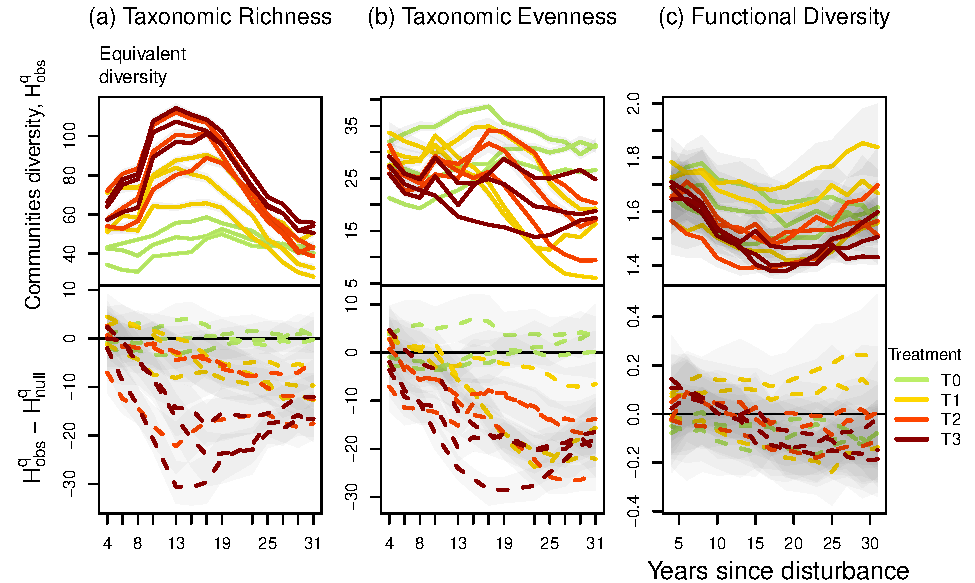
\includegraphics{RecruitmentTrajectories_files/figure-latex/DivTraj-1} 

}

\caption{Upper panels, trajectories over 30 years of rtaxonomic richness \textbf{(a)}, taxonomic evenness \textbf{(b)} and functional diversity \textbf{(c)} of 2-years laps recruitment. Lower panels, diversity differences to null models. Colors are treatments: green (control), yellow (T1), orange (T2), red (T3) with shaded areas the credibility intervals.}\label{fig:DivTraj}
\end{figure*}

\subsection{Functional composition}\label{functional-composition}

In undisturbed plots functional traits values remained stable over the
30 years while it followed hump-shaped trajectories in all disturbed
plots, to the exception of the leaf chlorophyll content. Trajectories of
SLA and bark thickness first increased before decreasing towards initial
values. Conversely, trajectories of leaf thickness, leaf toughness, wood
specific gravity, and maximum heigt first decreased and then started
returning towards initial values but their recovery remained unachieved
after 30 years (Figure \ref{fig:CWM}).

\begin{figure*}

{\centering 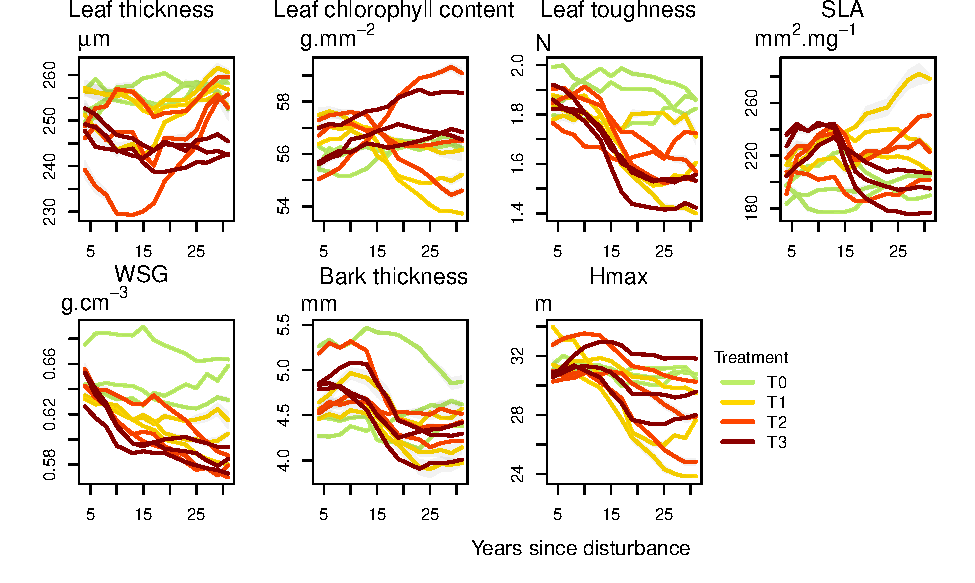
\includegraphics{RecruitmentTrajectories_files/figure-latex/CWM-1} 

}

\caption{Community weighted means (CWM) of the leaf, the two stem and specific maximum height. Colors are treatments: green (control), yellow (T1), orange (T2), red (T3) with shaded areas the credibility intervals.}\label{fig:CWM}
\end{figure*}

\subsection{Recruitment Turnover}\label{recruitment-turnover}

Over the 30 years in control plots the turnover of recruited species
compared to initial community remained low (Figure \ref{fig:Turnover}).
In disturbed plots the recruited species turnover followed a marked
hump-shaped trajectory, with a maximum reached around 15 years after
disturbance. The maximum turnover was positively correlated to the
disturbance intensity (\(\rho_{spearman}=0.93\)). Thirty years after
disturbance the turnover had returned to low values.

\begin{figure}

{\centering 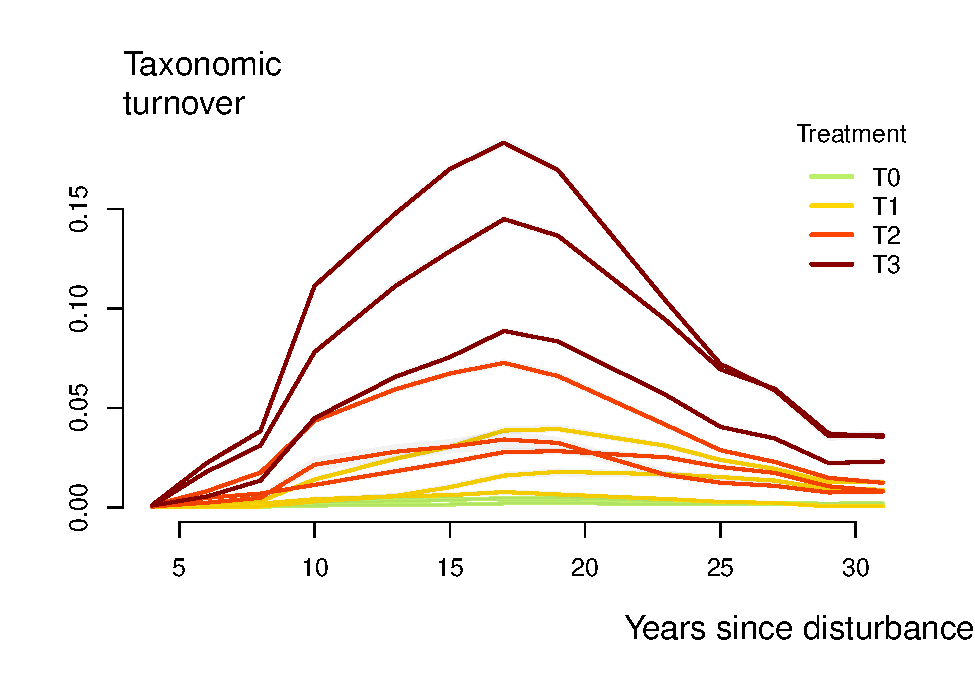
\includegraphics[width=1\linewidth]{RecruitmentTrajectories_files/figure-latex/Turnover-1} 

}

\caption{Trajectories over 30 years of the abundance-based turnover between 2-years laps recruited trees and initial communities before disturbance. Colors are treatments: green (control), yellow (T1), orange (T2), red (T3) with shaded areas the credibility intervals.}\label{fig:Turnover}
\end{figure}

\section{Discussion}\label{discussion}

\subsection{A three-phased deterministic successional
pathway}\label{a-three-phased-deterministic-successional-pathway}

Post-disturbance recruitment trajectories relied on a three-phased
successional pathway defined by the emergence of deterministic
competition processes for light gradually balancing the stochastic
recruitment specific to undistubed communities.

A first phase (0-8 years), corresponded to the recruitment of
pre-disturbance surviving saplings (DBH \textless{} 10cm) that
immediately benefited from the increased enlightment and alleviated
competition induced by disturbance \citep{Denslow2000, Herault2010}. The
taxonomic and functional characteristics of recruited trees mirrored the
pre-disturbance communities and recruitment processes matched the null
stochastic recruitment model.

A second phase (8-15 years) was marked by a shift in community
functional composition towards more ``acquisitive'' functional
strategies and the dominance of a restricted set of species. The
recruitment then involved true recruits, \emph{i.e.} trees germinated
from the seeds bank, representing the main part of the whole
post-disturbance recruitment \citep{Lawton1988}. The recruitment was
dominated by short-lived, fast growing hard pionneers highly competitive
and displaying efficient light acquisition
\citep{Wright2004, Chave2009b, Herault2011}. As already demonstrated in
temperate forests, the pool of recruited species was restricted by
trait-based competition processes selecting species with efficient light
acquisition (high SLA and leaf chlorophyll content) and inexpensive,
short-lived tissues (low leaf thickness and thoughness, small Hmax and
low wood specific gravity and bark
thickness)\citep{Chave2004, Kunstler2016}. This emergence of trait-based
deterministic processes balanced the stochastic recruitment observed in
the first place, and the relative importance of both processes was
determined by the disturbance intensity. After low intensity disturbance
(T1 plots) recruited species still mirrored pre-disturbance taxonomic
composition, but included more long-lived pioneers and light-demanding
species \citep{Bongers2009}. After intense disturbance in contrast (T2
and T3 plots), the composition of recruited trees rapidly differed from
pre-disturbance community and with the high dominance of hard pioneers,
such as Cecropia spp., likely entailing significant changes in
communities functioning \citep{Diaz2005}.

A third recruitment phase corresponded to the recovery of
pre-disturbance taxonomic and functional characteristics. Although the
recruits remained mainly light-demanding species their functional
diversity increased and they increasingly resembled resembled the
pre-disturbance taxonomic composition. The deterministic recruitment
processes then gradually left room to stochastic recruitment processes
specific to undisturbed forest \citep{Lawton1988, Chave2004}.

\subsection{The achievement of communities
recovery}\label{the-achievement-of-communities-recovery}

After disturbance the stochastic recruitment specific to undisturbed
communities was progressively restored and drove community taxonomic and
functional recovery. This confirmed previous results from the Paracou
experiment, conducted 10 years \citep{Molino2001} and 20 years
\citep{Baraloto2012a} after disturbance, where the early signs of the
resilience of taxonomic and functional composition had been detected.

Recruitment taxonomic richness and evenness recovered pre-disturbance
values and the taxonomic composition converged towards the
pre-disturbance community, thus maintaining the initial differences
among communities for all disturbance intensity. Community taxonomic
convergence revealed the scarce recruitment of species that did not
belong to pre-disturbance community, due to the commonness of dispersal
limitation among tropical tree species \citep{Svenning2005}.

Functional composition and diversity trajectories converged similarly in
the functional space towards the recovery of pre-disturbance values,
suggesting a common and resilient functioning despite communities'
taxonomic divergence \citep{Fukami2005}.

Trait-based selection processes made deterministic the community
functional response to disturbance but dispersal limitation and
steady-state stochastic recruitment made community taxonomic response
historically contingent. Although resilient, the functional and
taxonomic composition of recruited trees remained altered 30 years after
dissturbance by the dominance of light-demanding species. This long-term
impact specifically raises questions for the management of exploited
forests, as most valuable species are late-successional and would thus
require cutting cycles of more than 30 years \citep{Putz2012}.

\section{Conclusion}\label{conclusion}

The post-disturbance recruitment trajectories highlighted a three-phased
deterministic successional pathway shaped by the emergence of
competition processes for light balancing the stochastic recruitment of
undisturbed communities. The successional pathway first corresponded to
the enhanced growth of pre-disturbance surviving saplings mirroring the
taxonomic and functional charateristics of pre-disturbance communities.
Second, recruitment trajectories were shaped by true recruits from the
seeds bank selected through the emergence of competitive exclusion for
light fostering pioneer species. Above a disturbance intensity threshold
the second recruitment phase was dominated by short-lived hard pioneers
that drastically changed community composition, diversity and likely
functioning. A third phase eventually corresponded to the return towards
pre-disturbance recruitment composition and taxonomic and functional
diversity, through the recovery of stochastic recruitment processes
specific to undisturbed communities. Although resilient the recruitment
processes remained altered for more than 30 years, fostering more
pioneer and light-demanding species. This questioned the sustainability
and profitability of forest exploitation which mainly values
late-successional species that might be long to recover
\citep{Putz2012}. Besides, repeated disturbance might have increasingly
strong impacts, as community recovery involved the seeds bank and
probably altered the composition and diversity of the seeds stock
\citep{Norden2009}.

\begin{center}\rule{0.5\linewidth}{\linethickness}\end{center}

%----------------------------------------------------------------------------------------
%	REFERENCE LIST
%----------------------------------------------------------------------------------------

\bibliographystyle{mee}
\makeatletter
% The filename has .bib extension the must be eliminated
\filename@parse{references.bib}
% parse stores the file name in base. Extension starts at the first dot, so don't use dots in file names.
\bibliography{\filename@base}
\makeatother


%----------------------------------------------------------------------------------------

\end{document}
